
%%%%%%%%%%%%%%%%%%%%%%                                          About Style Transfer
\begin{frame}[fragile]{Neural Style Transfer}
   Style transfer relies on separating the content and style of an image. 
   \\
   Given one content image and one style image, we aim to create a new, target image which should contain our desired content and style components:
    \begin{itemize}
        \item objects and their arrangement are similar to that of the content image (feature reconstruction)
        \item style, colors, and textures are similar to that of the style image (texture synthesis)
    \end{itemize}

\end{frame}


%%%%%%%%%%%%%%%%%%%%%%                                         
\begin{frame}[fragile]{Neural Style Transfer}
    \begin{equation}
        content.image + style.image =  new.image with style.transfered
    \end{equation}
    \begin{figure}[ht]
      \hspace*{-1cm}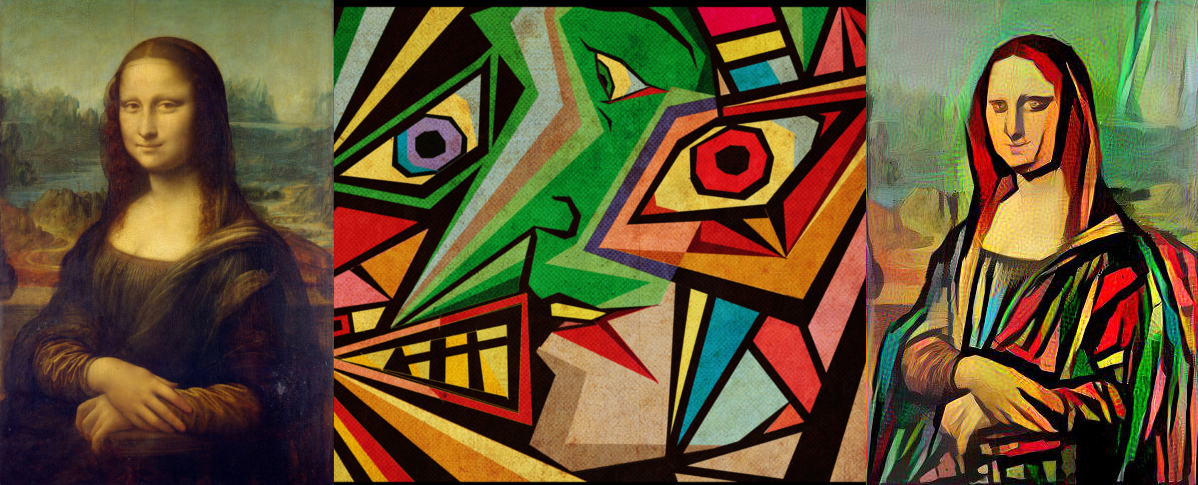
\includegraphics[width=0.5\linewidth]{styletransfer} \\
      \hspace*{-1cm}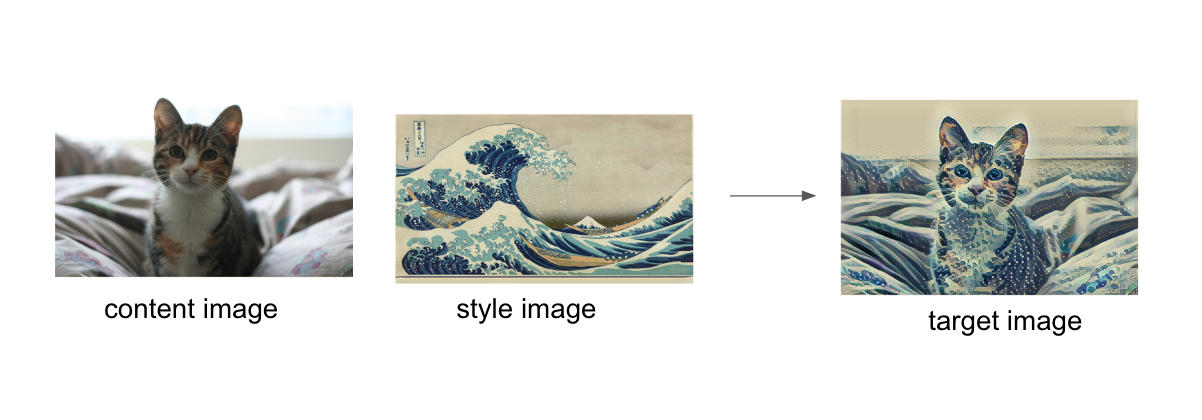
\includegraphics[width=0.7\linewidth]{styletransfercat} 
    \end{figure}
    https://github.com/puthusseri/styleTransfer.git
\end{frame}


%%%%%%%%%%%%%%%%%%%%%%%%%%%%%%%%%%%%%%%%%%%%%%%%%%